\documentclass{article}

\usepackage[utf8]{inputenc}
%\usepackage{a4wide}
\usepackage{amsthm}
\usepackage{amsmath}
\usepackage{url}
\usepackage{tikz}
\usetikzlibrary{topaths,calc}

\title{Modèles graphiques probabilistes}
\author{Charles-Pierre Astolfi, Émile Contal} 
\date{3 janvier 2012}

\begin{document}
\newtheorem*{mdef}{Définition}
\newtheorem*{mthm}{Théorème}

\maketitle

\begin{abstract}
Le but de notre travail est d'évaluer un algorithme qui permet
d'approximer la largeur arborescente (treewidth) d'un graphe.

Beaucoup de problèmes de graphes (par exemple, l'inférence bayesienne)
peuvent être résolus en temps polynomial sur des graphes de largeur
arborescente bornée. Le calcul exact de la largeur arborescente est un
problème NP-complet et nécessite l'utilisation d'heuristiques. Ce
rapport est dédié à l'étude d'un de ces algorithmes, décrit dans
\cite{rootpaper}.

\end{abstract}

\section{Introduction}
Dans le cadre de l'article ``A Practical Relaxation of Constant-Factor
Treewidth Approximation Algorithms'' \cite{rootpaper}, nous avons
implémenté l'algorithme proposé et l'avons comparé à d'autres
algorithmes de calcul de treewidth.


\section{Théorie}

Nous commençons cette section par quelques définitions qui nous seront
utiles dans la suite.

\begin{mdef}
Soit $G = (V,E)$ un graphe non-orienté sans boucle. On dit que $G$ est
connecté s'il existe un chemin entre chaque paire de sommets de $G$.
\end{mdef}

\begin{mdef}
On dit que $G$ est triangulé si pour tout cycle de longueur supérieure
strictement à 3, il existe une arête entre deux sommets non-adjacents
du cycle. La largeur d'un graphe triangulé est la taille de sa plus
grande clique moins 1.
\end{mdef}

\begin{mdef}
La largeur arborescente d'un graphe est la largeur minimale obtenable
parmi toutes les triangulations possibles.
\end{mdef}

\begin{mdef}
Un \emph{dtree} d'un graphe $G$ non-orienté est un arbre binaire
complet, dont les feuilles sont les arêtes de $G$.
\end{mdef}

\begin{mdef}
Le \emph{contexte} d'un noeud $t$ d'un dtree est l'ensemble des noeuds
qui représente le bord du sous-graphe $G(t)$ par rapport au graphe
$G$. C'est-à-dire qu'un noeud $v$ apparait dans le contexte de $t$ si
et seulement s'il y a $v-u$ dans $G$ avec $v$ dans $G(t)$ et $u$ hors
de $G(t)$.
\end{mdef}
Il permet de guider les algorithmes de partitionnement de type
\emph{divide-et-conquere}.

\begin{mdef}
Le \emph{cutset} d'un noeud $t$ d'un dtree est l'ensemble des noeuds
communs à $G(t_l)$ et à $G(t_r)$ et qui ne sont pas dans le contexte
de $t$.
\end{mdef}

Il est facile de vérifier que $context(t)$ et $cutset(t)$ sont des
ensembles disjoints, ce qui motive la définition suivante : 

\begin{mdef}
$$
cluster(t) = \left\{
    \begin{array}{ll}
        vars(t) & \mbox{ si $t$ est une feuille} \\
        cutset(t) \cup context(t) & \mbox{ sinon.}
    \end{array}
\right.
$$
\end{mdef}

Ceci permet de définir la largeur d'un $dtree$ : 
\begin{mdef}
La \emph{largeur} d'un dtree est la taille de son plus gros cluster
moins 1.
\end{mdef}

\begin{figure}[h!]
 \centering
\begin{tikzpicture}[auto, node distance=2cm]
  \node[] (1) {A};
  \node[below left of=1] (2) {B};
  \node[below right of=1] (3) {C};
  \node[below right of=2] (4) {D};
  \node[below right of=3] (5) {E};
 \path
  (1) edge node {} (2)
  (1) edge node {} (3)
  (2) edge node {} (3)
  (2) edge node {} (4)
  (3) edge node {} (4)
  (3) edge node {} (5);
\end{tikzpicture}
\caption{Exemple de graphe $G$}
\end{figure}

\begin{figure}[h!]
  \tikzstyle{internal} = [rectangle, draw]
  \tikzstyle{level 1} = [sibling distance=4cm]
  \tikzstyle{level 2} = [sibling distance=3cm]
  \tikzstyle{level 3} = [sibling distance=2cm]
  \tikzstyle{level 4} = [sibling distance=1.5cm]
  \centering
 \begin{tikzpicture}
    \node [internal] (0) {(\{B,C\}, \{\})}
    child{
      node [internal] (1) { (\{A\}, \{B,C\}) }
      child{
        node[] (2) { AB }
      }
      child{
        node[] (3) { AC }
      }
    }
    child{ 
      node [internal] (4) { (\{\}, \{B,C\}) }
      child{
        node[] (5) { CE }
      }
      child{
        node [internal] (6) { (\{\}, \{B,C\}) }
        child{
          node [] (7) {BC}
        }
        child {
          node [internal] (8)  { (\{D\}, \{B,C\}) }
          child{
            node[] (9) {CD}
          }
          child{
            node[] (10) {BD}
          }
        }
      }
    };
 \end{tikzpicture}
 \caption{Exemple de dtree du graphe $G$ avec les contextes et cutsets}
\end{figure}

\begin{figure}[h!]
  \centering

  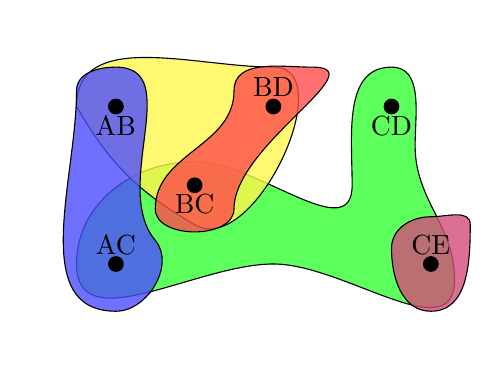
\begin{tikzpicture}
    \node (ab) at (0,2) {};
    \node (ac) at (0,0) {};
    \node (bc) at (1,1) {};
    \node (bd) at (2,2) {};
    \node (cd) at (3.5,2) {};
    \node (ce) at (4,0) {};

    \begin{scope}[fill opacity=0.8]
    \filldraw[fill=green!80] ($(ac)+(-0.5,0)$)
        to[out=90,in=180] ($(bc)+(0,0.3)$)
        to[out=0,in=270] ($(cd)+(-0.5,-1)$)
        to[out=90,in=180] ($(cd)+(0,0.5)$)
        to[out=0,in=90] ($(cd)+(0.3,-0.5)$)
        to[out=270,in=90] ($(ce)+(0.3,-0.2)$)
        to[out=270,in=0] ($(ce)+(-2,0)$)
        to[out=180,in=270] ($(ac)+(-0.5,0)$);
    \filldraw[fill=yellow!70] ($(ab)+(-0.5,0)$) 
        to[out=90,in=180] ($(bd) + (0,0.5)$) 
        to[out=0,in=330] ($(bc) + (0,-0.5)$)
        to[out=150,in=300] ($(ab)+(-0.5,0)$);
    \filldraw[fill=blue!70] ($(ab)+(-0.5,0.2)$)
        to[out=90,in=180] ($(ab)+(0,0.5)$)
        to[out=0,in=130] ($(ac)+(0.5,0.3)$)
        to[out=310,in=0] ($(ac)+(0,-0.6)$)
        to[out=180,in=270] ($(ab)+(-0.5,0.2)$);
    \filldraw[fill=red!70] ($(bd)+(-0.5,0.2)$)
        to[out=90,in=180] ($(bd)+(0.5,0.5)$)
        to[out=0,in=90] ($(bc)+(0.5,-0.3)$)
        to[out=270,in=270] ($(bc)+(-0.5,-0.3)$)
        to[out=90,in=270] ($(bd)+(-0.5,0.2)$);
     \filldraw[fill=purple!70] ($(ce)+(-0.5,0.2)$)
        to[out=90,in=180] ($(ce)+(0,0.6)$)
        to[out=0,in=90] ($(ce)+(0.5,0.5)$)
        to[out=270,in=0] ($(ce)+(0,-0.6)$)
        to[out=180,in=270] ($(ce)+(-0.5,0.2)$);
    \end{scope}

    \fill (ab) circle (0.1) node [below] {AB};
    \fill (ac) circle (0.1) node [above] {AC};
    \fill (bc) circle (0.1) node [below] {BC};
    \fill (bd) circle (0.1) node [above] {BD};
    \fill (cd) circle (0.1) node [below] {CD};
    \fill (ce) circle (0.1) node [above] {CE};
  \end{tikzpicture}
  \caption{Hypergraphe de $G$}
\end{figure}

Hopkins et Derwiche \cite{hop} ont proposé une transformation
polynomiale qui conserve la largeur entre les dtrees et les graphes
triangulés. C'est-à-dire qu'il est possible pour un graphe $G$ de
convertir une triangulation de $G$ de largeur $w$ en un dtree de
largeur $w$ et vice-versa. Cela donne ainsi une borne sur la largeur
arborescente de $G$.

Notre objectif est de donc construire un dtree de largeur la plus
petite possible ; pour ce faire on partitionne un hypergraphe $H(G)$
définit ainsi :
$$ H(G) = (E,\{ \{ (u,v) \in E \} \mid u \in V \}) $$

Le partitionnement de $H(G)$ est fait, comme dans l'article, grâce à
la librairie hMetis, qui utilise des heuristiques randomisées.

Robertson et Seymour \cite{robert} ont montré qu'il existait toujours
un partitionnement de $G(t)$ tel que chaque sous-graphe $G(t_l)$ et
$G(t_r)$ contiennent au plus $2/3$ des noeuds du contexte de $t$.  Un
tel partitionnement permet d'assurer que notre algorithme donnera une
approximation de la largeur arborescente d'au plus $4k+1$, avec $k$ la
largeur arborescente du graphe original.  En pratique, nous n'avons
aucune garantie de la part de hMetis de trouver un tel partitionnement
mais nos résultats expérimentaux montrent qu'on arrive à un facteur
$2$ de la treewidth.



\section{Implémentation}
Nous avons réalisé l'implémentation en OCaml \cite{ocaml}, et le code
est disponible à l'adresse
\url{http://www.dptinfo.ens-cachan.fr/~cpastolf/treewidth.zip}

Pour chaque execution du programme, de nombreuses approximations de la
treewidth sont faites, avec des paramètres pour hMetis différents.


\section{Résultats et discussion}
Tous nos test 

\bibliographystyle{amsplain}
\bibliography{biblio}

\end{document}
